\documentclass[aps,prxquantum,preprint,superscriptaddress,amsmath,amssymb]{revtex4-2}
\usepackage{graphicx}
\graphicspath{{./figures/}}
\usepackage{bm}
\usepackage{siunitx}
\usepackage{xcolor}
\usepackage{booktabs}
\usepackage{braket}
\usepackage[colorlinks=true, citecolor=blue, linkcolor=blue, urlcolor=blue]{hyperref}
\usepackage{xr-hyper}
\usepackage[capitalize, nameinlink]{cleveref}
\externaldocument[SI-]{si}
% --- Track C shared setup (siunitx, notation macros, cleveref names) ---
\sisetup{
  retain-unity-mantissa = false,
  exponent-product = \times
}
\setlength{\emergencystretch}{1.5em}
\DeclareSIUnit{\dB}{\deci\bel}

% --- Notation macros (identical in main text and Supplemental Material) ---
\providecommand{\mel}[3]{\langle #1 \vert #2 \vert #3 \rangle}
\providecommand{\ev}[1]{\langle #1 \rangle}
\newcommand{\Real}{\operatorname{Re}}
\newcommand{\Tr}{\operatorname{Tr}}
\newcommand{\Fnorm}{F_C^{\rm norm}}
\newcommand{\Fnormeff}{F_C^{\rm norm,eff}}
\newcommand{\Fraw}{F_C^{\rm raw}}
\newcommand{\Gfwd}{G_{\rm fwd}}
\newcommand{\Grev}{G_{\rm rev}}
\newcommand{\Iso}{\mathcal{I}}
\newcommand{\gNR}{\gamma_{\rm NR}}
\newcommand{\lint}{\lambda_{\rm inter}}

% --- cleveref: consistent, spelled-out cross-reference names ---
\crefname{equation}{Eq.}{Eqs.}
\Crefname{equation}{Equation}{Equations}
\crefname{table}{Table}{Tables}
\crefname{figure}{Fig.}{Figs.}
\Crefname{figure}{Figure}{Figures}
\crefname{section}{Sec.}{Secs.}

\begin{document}

\title{Spatial channel separation evades the single-port Petermann bound in a non-Hermitian optomechanical ladder}

\author{Juste Deuyekbe}
\affiliation{Department of Physics, Faculty of Science, University of Ngaoundere, P.O. Box 454, Ngaoundere, Cameroon}

\author{P. Djorw\'e}
\email{djorwepp@gmail.com}
\affiliation{Department of Physics, Faculty of Science, University of Ngaoundere, P.O. Box 454, Ngaoundere, Cameroon}
\affiliation{Stellenbosch Institute for Advanced Study (STIAS), Wallenberg Research Centre at Stellenbosch University, Stellenbosch 7600, South Africa}

\author{A.-H. Abdel-Aty}
\affiliation{Department of Physics, College of Sciences, University of Bisha, Bisha 61922, Saudi Arabia}

\author{A. Elrashidi}
\email{a.elrashidi@ubt.edu.sa}
\affiliation{College of Engineering, University of Business and Technology, Jeddah 21448, Saudi Arabia}

\author{Nsangou Mama}
\email{mnsangou@yahoo.com}
\affiliation{Department of Physics, Faculty of Science, University of Maroua, P.O.Box 46, Maroua, Cameroon}

\author{S. G. Nana Engo}
\email{serge.nana-engo@facsciences-uy1.cm}
\affiliation{Department of Physics, Faculty of Science, University of Yaounde I, P.O.Box 812, Yaounde, Cameroon}

\begin{abstract}
In single-port non-Hermitian sensors the Petermann factor offsets susceptibility gains and bounds metrological precision. Can this penalty be bypassed? We show that it can, and that the bound is architectural, not fundamental. A two-port double-chain optomechanical ladder with opposing non-reciprocal hoppings, and hence opposing skin-effect directions, separates signal amplification from quantum-noise drainage. Its operating points form a precision--gain frontier controlled by the spectral margin: the deep-stability class has median homodyne-record $\Fnorm=\num{0.928}$ over \num{60} independent restarts, and the marginal class has median $\Gfwd=+\qty{14.5}{\dB}$ at $\Fnorm=\num{0.063}$. Gradient-based differentiable optimal control maximizes the resource-normalized Fisher information $\Fnorm$ under a Hurwitz-stability constraint. For $N\in\{\num{6},\dots,\num{16}\}$ the optimizer returns $\Fnorm>0$ in two initialization-dependent classes at opposite ends of the frontier: deep stability with $\Fnorm\in\numrange{0.937}{0.987}$ and attenuated transmission, and marginal stability with directional gain $\Gfwd\in\qtyrange{13.5}{15.5}{\dB}$ and isolation $\qtyrange{40}{64}{\dB}$. The two classes coexist at every size. All solutions stay Hurwitz-stable under \qty{5}{\percent} disorder (\qty{87.5}{\percent} recovery), and the deep-stability advantage survives realistic preamplifier noise at $\Fnormeff\approx\num{0.3}$--$\num{0.5}$.
\end{abstract}

\maketitle

\section{Introduction}
\label{sec:intro}

Non-Hermitian physics hosts phenomena with no counterpart in closed Hermitian systems, and open quantum systems provide a natural setting in which to realize them~\citep{Yao2018,Bergholtz2021,ElGanainy2018,Ashida2020,Feng2017,Rotter2017}. A paradigmatic example is the non-Hermitian skin effect (NHSE): under open boundary conditions, a macroscopic fraction of the bulk eigenstates of a non-reciprocal lattice localizes exponentially at the system boundary~\citep{Yao2018,Schomerus2020,Weidemann2020,Helbig2020,GhatakDas2019}, in stark departure from Bloch-band intuition and from the conventional bulk-boundary correspondence~\citep{Peano2015,Kunst2018}. In a related but distinct line of work, systems tuned close to an exceptional point display a strongly enhanced susceptibility to external perturbations~\citep{Hodaei2017,Wiersig2020,Ozdemir2019,MiriAlu2019,Langbein2018}, a property that has motivated sustained interest in non-Hermitian sensing platforms.

This metrological gain is not free. Near an exceptional point the relevant eigenvectors coalesce, and their growing non-orthogonality amplifies quantum projection noise: a cost captured quantitatively by the Petermann factor $K$~\citep{Zhang2019}. Lau and Clerk~\citep{Lau2018}, together with a series of subsequent analyses~\citep{Duggan2022,McDonald2020,McDonald2020Exponential,Bao2021,Ding2023}, showed that once the total intracavity photon occupancy is correctly accounted for as the metrological resource~\citep{Braunstein1994,Giovannetti2011,Demkowicz2012}, this excess noise exactly offsets the apparent susceptibility gain in single-port architectures: the resource-normalized Fisher information saturates or decays with the very parameters that enhance the raw susceptibility. These single-port limits were recently reviewed from the quantum-Fisher-information perspective~\citep{Wiersig2026}. On the noise-metric side, a passive cavity-magnonic system reports a twelve-fold signal-to-noise enhancement at a third-order coherent-perfect-absorption exceptional point~\citep{Wang2026}, and a unified theory of transmission peak degeneracies supplies analytic figures of merit that avoid the eigenbasis-collapse noise amplification limiting exceptional-point sensors~\citep{Carney2026}. On the Fisher-information side, recent analyses of non-Hermitian lattices~\citep{LiGuo2026,Wu2026CQFI,Liang2026,XieXu2024} address eigenvalue-shift sensitivity, covariant bounds, Green's-function amplification, and few-mode nonreciprocal couplings, but none reports the measurement-record information normalized by total two-chain occupancy under stability-constrained optimization.

The central question is therefore: \emph{can a multi-port architecture with opposing skin directions evade the single-port Petermann bound under full two-chain photon accounting, by separating where photons are consumed from where the signal is read out rather than by suppressing the underlying noise?} The answer, established below, is that it can: at a quantifiable precision--gain cost controlled by the spectral margin, not as a universal enhancement.

We address this question with a double-chain ladder built from two engineered directional non-reciprocal chains~\citep{Metelmann2015,Fang2017,Peterson2017,Kongkui2024,Berinyuy2025}. Two nominally identical chains, biased toward opposite skin directions, are coupled weakly to one another: chain~A concentrates the signal response at a designated read-out port, while chain~B drains the Langevin fluctuations of the joint system toward the opposite boundary. The metrological resource is counted across \emph{both} chains, so no photon is hidden from the normalization, yet the signal itself is spatially segregated from the bulk of the fluctuations. We optimize this architecture with gradient-based, differentiable optimal control (DOC), maximizing the continuous measurement-record Fisher information subject to a strict Hurwitz-stability constraint. The resulting parameter landscape supports two physically distinct operating regimes, one optimized for per-photon precision, the other for directional gain, and the two regimes sit at opposite ends of a continuous frontier rather than realizing a single universal operating point. Both remain Hurwitz-stable in the tested disorder study, while precision retention is quantified for a finite restart ensemble below.

\section{Physical framework and methods}
\label{sec:methods}

We consider a one-dimensional array of $N$ coupled single-mode cavities with uniform decay rate $\kappa$. Non-reciprocal hopping between neighboring sites is parameterized asymmetrically as $J_R=Je^{+g}$ and $J_L=Je^{-g}$, so the associated non-reciprocal rate is $\gNR=2J\sinh(g)$; the target operating regime throughout is $\gNR/\kappa\ge\num{2}$, which supports well-developed skin-mode localization.

For a single chain under open boundary conditions, the linear drift matrix in the cavity-mode basis reads
\begin{equation}\label{eq:obc_drift}
A(\theta)=-\kappa\,\mathbb{I}_N-iH_{\rm NHSE}(\theta),
\end{equation}
where the non-Hermitian Hamiltonian $H_{\rm NHSE}$ carries a boundary parameter $\theta=\theta_0+\Delta\theta$ that plays the role of the unknown signal to be estimated, with fiducial value $\theta_0=\qty{0.1}{\kappa}$ and perturbation $\Delta\theta=\num{1e-3}\kappa$.

The double-chain ladder couples two such chains, biased toward opposite skin directions, through a uniform inter-chain matrix $\Lambda=\lint e^{i\phi}\mathbb{I}_N$. The joint $2N\times2N$ drift matrix of the ladder reads
\begin{equation}\label{eq:ladder_drift}
A_{\rm ladder}(\theta)=
\begin{pmatrix}
A_A(\theta) & \Lambda \\
\Lambda^\dagger & A_B
\end{pmatrix}.
\end{equation}
Working in the real quadrature representation, the stationary covariance matrix $\Sigma$ of the joint system obeys the continuous Lyapunov equation under vacuum noise injection, and the continuous Gaussian measurement-record Fisher information for homodyne detection follows as
\begin{equation}\label{eq:record_fisher}
F_C=(\partial_\theta\bm{\mu})^{T}\Sigma^{-1}(\partial_\theta\bm{\mu})+\frac{1}{2}\Tr\!\bigl[(\Sigma^{-1}\partial_\theta\Sigma)^2\bigr],
\end{equation}
where $\bm{\mu}=-\mathcal{A}_{\rm real}^{-1}\bm{u}_{\rm in}$ is the steady-state quadrature displacement. Resource normalization is performed with respect to the \emph{total} photon occupancy summed over both chains,
\begin{equation}\label{eq:norm}
\Fnorm=\frac{F_C}{\|\bm{\mu}\|^2},
\qquad
\|\bm{\mu}\|^2=\sum_{j=1}^{N}\Bigl(\bigl|\braket{a_j}\bigr|^2+\bigl|\braket{b_j}\bigr|^2\Bigr),
\end{equation}
so any advantage reported below cannot be attributed to hiding photons outside the counted resource. Because the left and right eigenvectors of the joint drift matrix enter the covariance $\Sigma$ and the mean response $\bm{\mu}$ through the full $2N$-dimensional spectrum, the Petermann factor associated with individual modes does not cancel the normalized information once the signal is spatially segregated from the bulk of the fluctuations. The numerator $F_C$ is dominated by the local response at the designated read-out port of chain~A, while the denominator counts photons on both chains. This architectural separation is what allows $\Fnorm$ to remain strictly positive, in contrast to the single-port cancellation derived by Lau and Clerk~\citep{Lau2018} and by McDonald and Clerk~\citep{McDonald2020}. Directional transmission is obtained from the scattering matrix $S=\mathbb{I}-\sqrt{2\kappa}\,A_{\rm ladder}^{-1}$~\citep{Clerk2010}; forward and reverse gains follow as $\Gfwd=10\log_{10}|S_{N,1}|^2$ and $\Grev=10\log_{10}|S_{1,N}|^2$, with isolation defined as $\Iso=\Gfwd-\Grev$.

Parameter optimization is carried out with automatic differentiation in JAX~\citep{Bradbury2018} and the Adam optimizer~\citep{Kingma2014,Leung2017}, maximizing $\Fnorm$ subject to a strict Hurwitz-stability barrier $\max\Real\lambda<\num{-0.05}$, enforced throughout the optimization rather than checked \emph{post hoc}. The Petermann factor $K$ and the biorthogonal QFI $F_Q^B$ serve as diagnostics only; $K$ does not enter the optimized estimand $\Fnorm$ (\cref{eq:norm}). Throughout, $\Fnorm$ denotes an achievable homodyne-record information under resource normalization, distinct from an ultimate covariant bound or from an eigenvalue-shift sensitivity per noise amplitude. The underlying Gaussian/Lyapunov machinery was cross-validated against independent open-system implementations on a shared dissipative-Rabi benchmark: the record mean agrees with the exact master-equation solution within statistical error, and independent propagators agree to $\num{4e-14}$.

\section{Results}
\label{sec:results}

\subsection{Single-chain baseline}
\label{sec:single}

We first establish the single-port baseline that the double-chain architecture is designed to surpass. \cref{fig:setups}(a) shows the single-chain ring configuration used for this baseline characterization. In the single-chain geometry, at fixed $J=\qty{0.5}{\kappa}$ and $g=\num{1.7}$ ($\gNR/\kappa=\num{2.646}$), both the matched boundary signal-to-noise ratio and the raw Fisher information grow exponentially with system size:

\begin{figure}[htpb]
\centering
\begin{minipage}[c]{0.49\columnwidth}
\centering
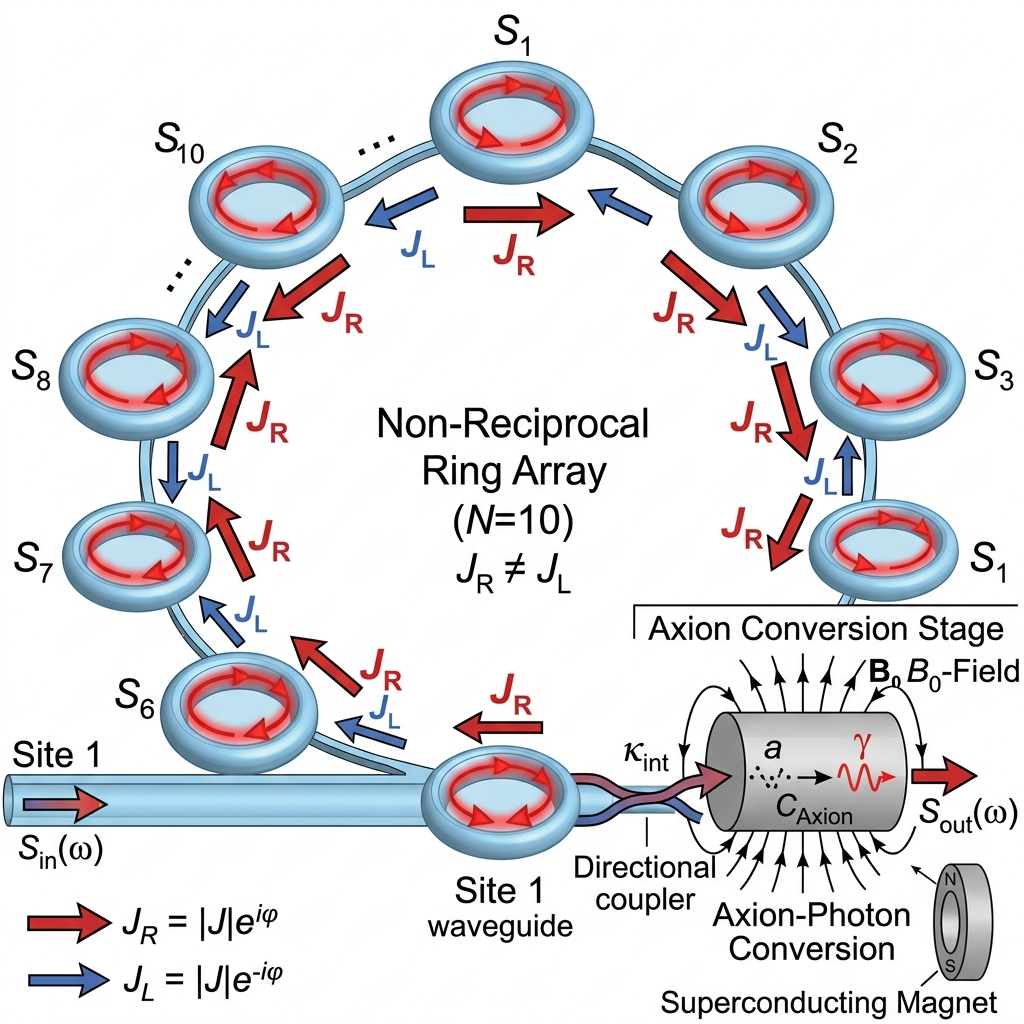
\includegraphics[width=\linewidth]{ring_setup.png}\\
(a)
\end{minipage}\hfill
\begin{minipage}[c]{0.49\columnwidth}
\centering
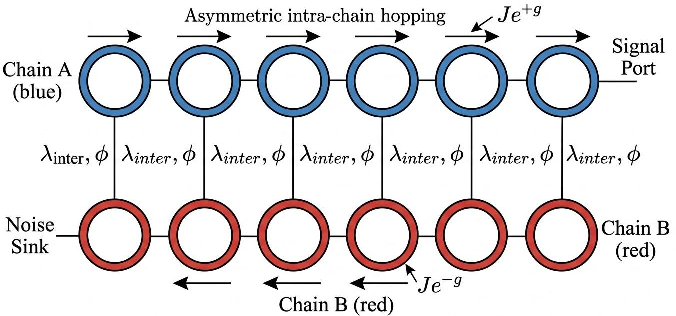
\includegraphics[width=\linewidth]{double_chain_setup.pdf}\\
(b)
\end{minipage}
\caption{Sensor geometries. (a)~Single-chain ring baseline: $N$ coupled cavity sites with non-reciprocal hopping $J e^{\pm g}$ and uniform dissipation $\kappa$; the boundary signal is injected at site~$j=N$ and the matched read-out port collects the amplified response. (b)~Double-chain ladder: chains A and B carry opposing non-reciprocal hoppings and are weakly coupled by $\Lambda=\lint e^{i\phi}\mathbb{I}_N$; the signal perturbation is applied at site $N$ of chain~A while Langevin noise is drained toward site~1 of chain~B.}
\label{fig:setups}
\end{figure}
\begin{align}
\ln(\mathrm{SNR}_N)&=a_{\rm snr}N+b_{\rm snr}, &
a_{\rm snr}&=+\num{0.1723}, & R^2&=\num{0.9843},
\label{eq:snr_fit}\\
\ln(\Fraw)&=a_{\rm raw}N+b_{\rm raw}, &
a_{\rm raw}&=+\num{2.4616}, & R^2&=\num{0.9992}.
\label{eq:fraw_fit}
\end{align}
Resource normalization by the intracavity photon number, however, reverses the trend and yields a \emph{negative} slope,
\begin{equation}\label{eq:fnorm_fit}
\ln(\Fnorm)=a_{\rm norm}N+b_{\rm norm},
\qquad
a_{\rm norm}=-\num{0.7625},\quad R^2=\num{0.9964}.
\end{equation}
The internal photon occupancy accumulates faster than the raw Fisher information can compensate, precisely recovering the single-port resource bound of Lau and Clerk~\citep{Lau2018} and of McDonald and Clerk~\citep{McDonald2020} (\cref{fig:single_vs_double}). Even after DOC restricted to the single-chain parameters $(J,g)$, the normalized Fisher information remains of order $10^{-3}$, more than two orders of magnitude below the deep-stability double-chain values reported in \cref{sec:double}. The full $N$-scaling data are tabulated in \cref{SI-tab:si_single} of the Supplemental Material.

\begin{figure}[htpb]
\centering
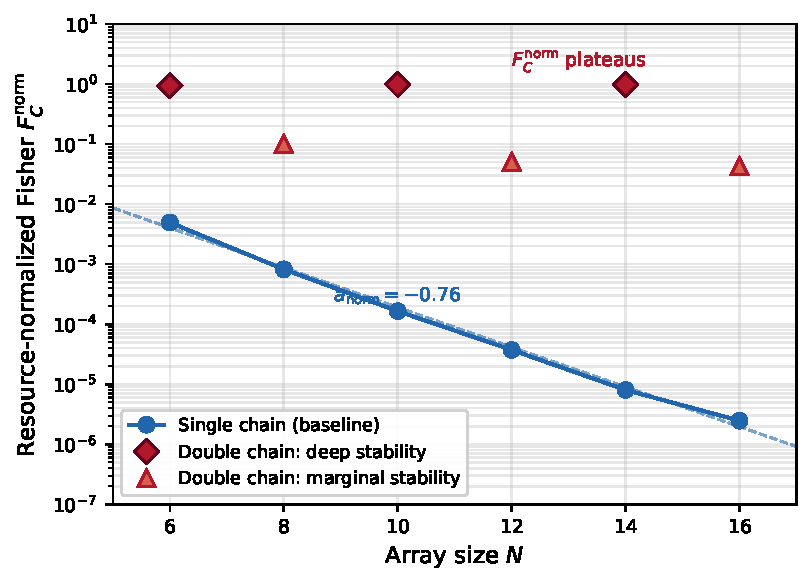
\includegraphics[width=0.8\columnwidth]{single_vs_double_chain_norm.pdf}
\caption{Resource-normalized Fisher information $\Fnorm$ versus array size $N$ for the single-chain (blue, $J=\qty{0.5}{\kappa}$, $g=\num{1.7}$) and double-chain ladder (red, DOC-optimized) architectures. The single-chain exhibits a negative scaling slope ($a_{\rm norm}=-\num{0.7625}$), while the double-chain achieves $\Fnorm>0$ for all $N\in\numrange{6}{16}$; the apparently flat single-chain tail at large $N$ is a linear-scale artifact, the semilog fit of \cref{eq:fnorm_fit} decays exponentially.}
\label{fig:single_vs_double}
\end{figure}

\subsection{Double-chain ladder and channel separation}
\label{sec:double}

The ladder geometry [\cref{fig:setups}(b)] assigns opposing skin directions to the two chains (\cref{fig:skin_modes}). Chain~A localizes toward the read-out port at site $j=N$, while chain~B localizes toward the noise sink at site $j=1$, realizing a spatial separation of signal and noise channels unavailable in any single-port architecture. The optimized inter-chain couplings span the moderate range $\lint/J\in\numrange{0.07}{1.02}$ (\cref{tab:nscaling}); only the largest lattices operate in the perturbative weak-evanescent limit invoked to avoid the mode delocalization reported experimentally for strongly coupled NHSE chains~\citep{Wang2025}, and outside that limit the separation of signal and noise channels is protected empirically by the stability barrier enforced throughout the optimization. In absolute units, the same optimal couplings ($\lint\in\numrange{0.016}{0.079}\kappa$) remain compatible with evanescent near-field overlap between parallel silicon phononic-crystal nanobeams~\citep{MacCabe2020} at a lithographic gap $d\approx\qty{400}{\nano\meter}$: at $\kappa/2\pi=\qty{1.7}{\mega\hertz}$ this yields $\lint/2\pi$ from \qty{27} to \qty{134}{\kilo\hertz}, achievable with current nanofabrication tolerances. The DOC-optimized inter-chain phase $\phi$ is size-dependent, spanning $\phi\in\numrange{1.35}{5.15}\,\mathrm{rad}$ across the six solutions of \cref{tab:nscaling} and clustering near neither $0$ nor $\pi/2$; whatever the operating value, it is held in practice by a synthesized Kuramoto synchronization potential~\citep{Asano_2025} (detailed in \cref{SI-eq:si_kuramoto}), which locks the relative phase against thermal crosstalk and slow drift.

\begin{figure}[htpb]
\centering
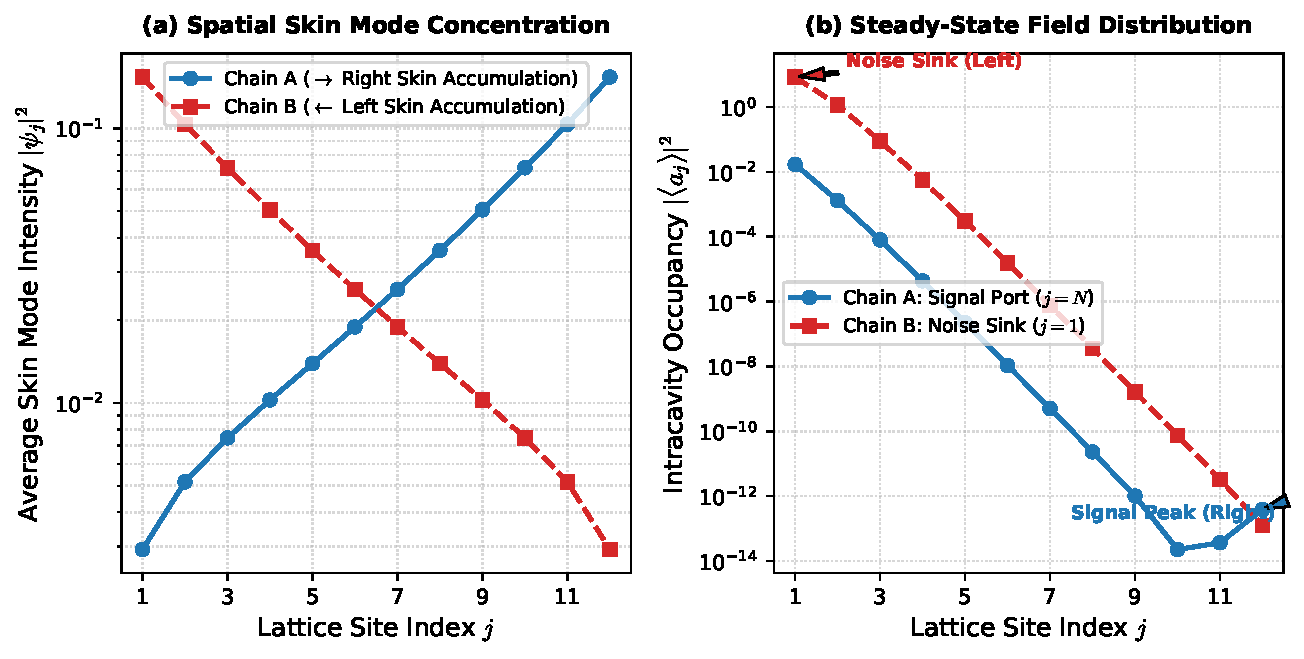
\includegraphics[width=0.85\columnwidth]{trackC_multichain_spatial_skin_modes.pdf}
\caption{Spatial skin-mode concentration in the double-chain ladder ($N=\num{12}$). (a)~Normalized eigenmode intensity $|\psi_j|^2$: rightward localization in Chain~A (signal port, $j=N$), leftward localization in Chain~B (noise sink, $j=1$). (b)~Steady-state field occupancy under single-port driving, showing asymmetric routing that isolates the read-out port from bulk quantum noise.}
\label{fig:skin_modes}
\end{figure}

A bare grid scan at fixed hoppings shows that strong inter-chain coupling destabilizes the joint spectrum. Multi-parameter DOC over $(J,g,\lint,\phi)$ restores stability throughout the accessible range and produces the $N$-dependent performance summarized in \cref{tab:nscaling}.

\begin{table}[htpb]
\caption{DOC-optimized double-chain performance across system size. Each row is one representative frontier endpoint per size (initialization-selected in 32/60 restarts of the six-size ensemble, $\approx\qty{53}{\percent}$; row alternation illustrative, not parity physics). All entries satisfy $\max\Real\lambda<\num{-0.05}$. Isolation is $\Iso=\Gfwd-\Grev$.}
\label{tab:nscaling}
\begin{ruledtabular}
\begin{tabular}{S S S S S S S}
{$N$} & {$J/\kappa$} & {$g$} & {$\lint/\kappa$} & {$\Fnorm$} & {$\Gfwd$~[\si{\dB}]} & {$\Iso$~[\si{\dB}]} \\
\hline
6  & 0.105 & 1.250 & 0.0164 & 0.937 & -40.1  & 69.6 \\
8  & 0.354 & 0.973 & 0.0695 & 0.101 & +13.5  & 40.5 \\
10 & 0.078 & 1.001 & 0.0790 & 0.984 & -117.3 & 41.5 \\
12 & 0.345 & 1.024 & 0.0278 & 0.050 & +15.5  & 56.9 \\
14 & 0.087 & 0.797 & 0.0775 & 0.987 & -181.3 & 40.4 \\
16 & 0.287 & 1.226 & 0.0207 & 0.043 & +14.3  & 64.0 \\
\end{tabular}
\end{ruledtabular}
\end{table}

Two solution classes appear; which one is selected correlates with lattice size and with optimizer initialization (quantified below):
\begin{itemize}
\item \textbf{Deep-stability class} ($N=\numlist{6;10;14}$). The optimizer converges to strong damping ($\max\Real\lambda\approx\num{-0.70}\kappa$) with comparatively low hopping and high normalized Fisher information, $\Fnorm\in\numrange{0.937}{0.987}$. Forward transmission is strongly attenuated ($\Gfwd$ ranging from $\qty{-40}{\dB}$ to $\qty{-181}{\dB}$), while reverse isolation remains high, $\Iso\in\qtyrange{40}{70}{\dB}$ (the maximum, $\qty{69.6}{\dB}$, occurs at $N=\num{6}$). This regime maximizes per-photon precision at the expense of signal throughput. Because the output power is suppressed by many orders of magnitude, a quantum-limited preamplifier (e.g., a Josephson parametric amplifier) at the read-out port is indispensable for practical detection; without it, the deep-stability advantage remains purely metrological. In short, the tabulated deep rows require a JPA stage at the read-out port, leaving $\Fnormeff\approx\num{0.3}$--$\num{0.5}$ (preamplifier photons downstream of the read-out port do not enter $\|\bm{\mu}\|^2$).

\item \textbf{Marginal-stability class} ($N=\numlist{8;12;16}$). The system instead operates close to the stability boundary ($\max\Real\lambda\approx\num{-0.06}\kappa$) with larger hopping. A net forward gain emerges, $\Gfwd\in\qtyrange{13.5}{15.5}{\dB}$, together with isolation of $\qtyrange{40}{64}{\dB}$, while $\Fnorm$ remains positive but modest, $\Fnorm\in\numrange{0.043}{0.101}$. This regime is best suited to directional preamplification rather than to precision metrology; the lowest $\Fnorm$ values ($\sim\num{0.04}$) remain one to two orders of magnitude above the single-chain baseline ($\sim\num{1e-3}$) but are nevertheless noise-dominated in absolute terms. Directional gain here is classical signal boost subject to amplifier quantum limits, not metrological information gain.
\end{itemize}

The physical origin of the deep-stability advantage is instructive: strong damping ($\max\Real\lambda\approx\num{-0.70}\kappa$) suppresses the covariance matrix $\Sigma$, and hence the quantum projection noise, while the skin effect simultaneously concentrates the mean displacement $\bm{\mu}$ at the read-out port of chain~A. The resource normalization counts photons on \emph{both} chains, but the signal photons reside predominantly in chain~A whereas the noise photons are distributed across the full ladder; the net effect is that the denominator $\|\bm{\mu}\|^2$ grows more slowly than the Fisher information $F_C$, driving $\Fnorm$ toward unity. In the marginal-stability class the weaker damping ($\max\Real\lambda\approx\num{-0.06}\kappa$) leaves a larger residual covariance, so the noise grows faster than the signal and $\Fnorm$ remains modest. The two classes thus realize a concrete precision--gain trade-off rather than a uniform improvement over the single-chain baseline.

To map this trade-off across the spectral margin, we aggregate all converged solutions from the multi-restart DOC ensemble (\num{10} independent initializations per size, primary protocol) together with the six published optima of \cref{tab:nscaling}. The resulting cloud of operating points (\cref{fig:tradeoff}) confirms that the two discrete classes occupy opposite ends of a clear frontier: $\Fnorm$ remains near unity for $\max\Real\lambda\lesssim-\num{0.4}\kappa$ and is modest near the Hurwitz boundary, while $\Gfwd$ simultaneously rises from strongly attenuated values to a net directional gain of order \qty{15}{\dB}. Isolation remains substantial ($\Iso\gtrsim\qty{35}{\dB}$, median $\approx\qty{53}{\dB}$) across the entire margin. The published solutions of \cref{tab:nscaling} (open black circles) lie on this frontier, showing that the DOC basins select different operating points along the same underlying precision--gain continuum. Across \num{60} independent restarts the typical (median) operating points are $\Fnorm=\num{0.928}$ (interquartile $\numrange{0.903}{0.976}$) for the deep class and $\Fnorm=\num{0.063}$ (interquartile $\numrange{0.044}{0.098}$) with $\Gfwd=+\qty{14.5}{\dB}$ (interquartile $+\qtyrange{10.7}{22.7}{\dB}$) for the marginal class, with median isolation \num{50.2} and \num{53.0}~dB respectively; the tabulated optima therefore sit at the frontier edge, while the medians describe typical draws. For comparison, off-exceptional-deficiency operation preserves exponential sensitivity at reduced prefactor with linear signal-to-noise scaling~\citep{LiGuo2026}; here the control knob is instead the spectral margin via constrained optimization, and the cost function is the resource-normalized record information.

\begin{figure}[htpb]
\centering
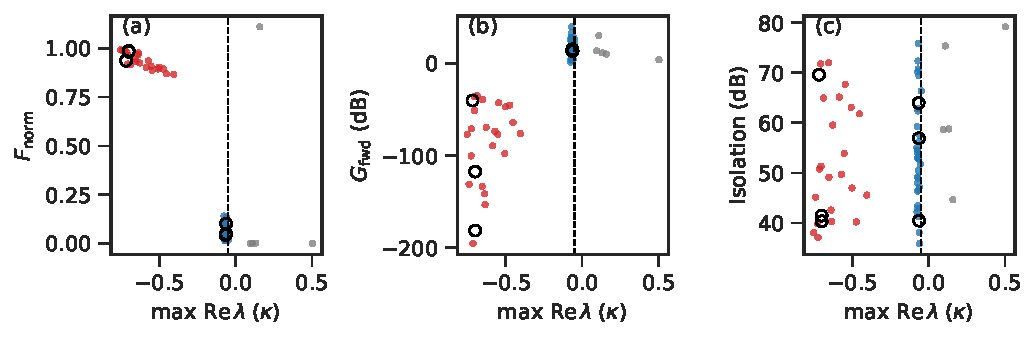
\includegraphics[width=0.92\columnwidth]{tradeoff_stability_margin.pdf}
\caption{Precision--gain trade-off across the stability margin. (a)~Resource-normalized Fisher information $\Fnorm$, (b)~forward gain $\Gfwd$, and (c)~isolation $\Iso$ versus the spectral abscissa $\max\Real\lambda$. Red (blue) markers are deep-stability (marginal-stability) solutions, gray markers unstable draws, obtained from the multi-restart DOC ensemble across $N\in\{\num{6},\dots,\num{16}\}$; open black circles highlight the six published optima of \cref{tab:nscaling}. The vertical dashed line marks the primary stability threshold $\max\Real\lambda=-\num{0.05}\kappa$.}
\label{fig:tradeoff}
\end{figure}

Beyond the six-point $N$-scan of \cref{tab:nscaling}, we additionally characterize a single reference configuration at $N=\num{12}$ chosen to probe the Petermann-factor regularization independently ($J=\qty{0.138}{\kappa}$, $g=\num{2.055}$, $\lint=\qty{0.010}{\kappa}$, $\phi=\num{1.736}\,\mathrm{rad}$; see \cref{SI-tab:si_petermann_sensitivity}). At this point the scattering matrix yields forward gain $\Gfwd=\qty{+12.1}{\dB}$, reverse gain $\Grev=\qty{-67.2}{\dB}$, and peak directional isolation of $\qty{79.3}{\dB}$, larger than any $N=\num{12}$ value in \cref{tab:nscaling} (which was optimized for $\Fnorm$ rather than for isolation). This illustrates that the architecture supports a wider range of operating points than the single representative optimum per size in the table.

\subsection{Disorder resilience and convergence}
\label{sec:disorder}

Fabrication imperfections inevitably perturb the nominally identical detunings and hoppings assumed above; we therefore stress-test the optimized solutions against static disorder. Under uncorrelated Gaussian disorder of root-mean-square amplitude $\sigma_{\rm RMS}=\qty{0.05}{\kappa}$ (i.e., approximately \qty{5}{\percent} fluctuations on detunings and hoppings), we re-optimize each of 16 independent realizations with a multi-restart DOC protocol (differential-evolution global search followed by Adam refinement, spectral margin $\Delta=\num{0.05}\kappa$) about a dedicated strongly coupled reference configuration $(J,g,\lint,\phi)\approx(\num{0.05}\kappa,\ \num{2.05},\ \num{0.52}\kappa,\ \pi/2)$, architecturally distinct from the \cref{tab:nscaling} entries (whose $\lint$ values are several-fold smaller) and documented in \cref{SI-sec:si_disorder}. At least \qty{80}{\percent} of the nominal $\Fnorm$ is recovered in 14 of 16 realizations (pass threshold 12 of 16), with mean retention \qty{164.9}{\percent}~$\pm$~\qty{47.1}{\percent}, retention ratios above \qty{200}{\percent} capped at \qty{200}{\percent} in the statistics, and all 16 re-optimized solutions Hurwitz-stable. The two failing realizations saturate the lower search boundary $g=\num{0.5}$ at inter-chain ratios $\lint/J\in\numrange{3.3}{6.3}$: they are optimization artifacts of the search domain rather than genuine dynamical fragility (\cref{SI-sec:si_disorder}).

Independently, bosonic master-equation simulations on a $3\times4$ Fock-cutoff grid confirm that the extracted dynamical rates are free of truncation artifacts once the cutoff satisfies $n_{\rm cut}\ge4$.

\begin{figure}[htpb]
\centering
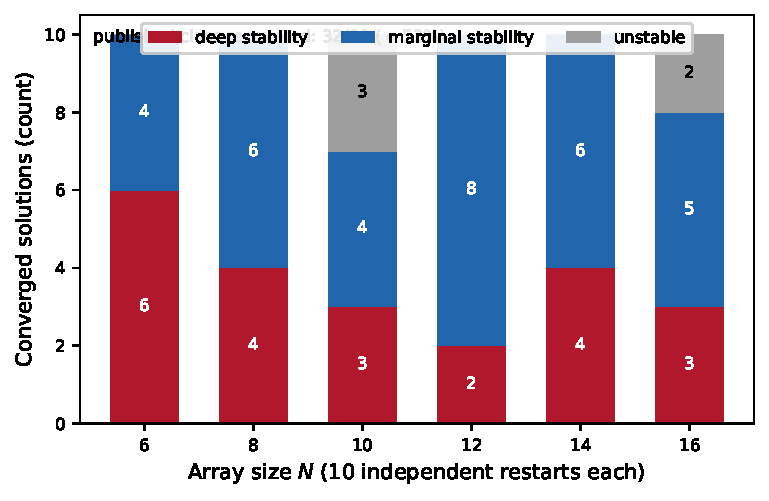
\includegraphics[width=0.95\columnwidth]{optimization.pdf}
\caption{Initialization dependence of the DOC solution landscape. Ten independent re-optimizations per ladder size under the primary protocol are classified as deep-stability (red), marginal-stability (blue), or unstable (gray). The tabulated class of \cref{tab:nscaling} coincides with the basin reached in 32 of 60 cases ($\approx\qty{53}{\percent}$): both basins coexist across sizes, and class selection is governed by initialization rather than by lattice parity (\cref{sec:discussion}).}
\label{fig:doc_trajectories}
\end{figure}

\section{Discussion}
\label{sec:discussion}

The double-chain architecture implements a deliberate precision--gain trade-off rather than a universal enhancement over the single-port baseline. The multi-restart ensemble of \cref{fig:tradeoff} shows that the two discrete classes of \cref{tab:nscaling} are the endpoints of the same precision--gain frontier controlled by the spectral margin $\max\Real\lambda$; the tabulated class is one representative optimum per size, selected in $\approx\qty{53}{\percent}$ of independent restarts. Deep-stability operation ($N=\numlist{6;10;14}$) achieves per-photon Fisher information near unity, $\Fnorm\approx\numrange{0.94}{0.99}$, by sitting deep within the stable regime ($\max\Real\lambda\approx\num{-0.70}\kappa$) and suppressing forward transmission. This regime is best suited to high-precision metrology, where shot-noise-limited sensitivity dominates over the requirement of high signal throughput; a quantum-limited preamplifier is then required to recover the attenuated output, after which the effective information remains $\Fnormeff\approx\num{0.3}$--$\num{0.5}$.

The marginal-stability class ($N=\numlist{8;12;16}$), by contrast, sits near the Hurwitz boundary ($\max\Real\lambda\approx\num{-0.06}\kappa$) and delivers $\Gfwd\approx\qtyrange{13.5}{15.5}{\dB}$ with isolation $\approx\qtyrange{40}{64}{\dB}$, while retaining a modest but strictly positive $\Fnorm\in\numrange{0.043}{0.101}$. This configuration functions naturally as a directional preamplifier, boosting weak signals before downstream noise sources come to dominate. The margin tradeoff has an independent eigenbasis signature: the maximum Petermann factor over the drift spectrum is modest and flat in the deep class ($K_{\max}\approx\num{12}$--$\num{17}$) but grows with system size in the marginal class ($\num{7.8}\to\num{31}\to\num{58}$ at $N=\num{8},\num{12},\num{16}$), placing the gain class progressively closer to exceptional-point operation while the precision class stays far from it; the gain-versus-Petermann-noise tradeoff is thus resolved as a size-dependent frontier, computed from the biorthogonal eigensystem at the tabulated optima. Read against the unified theory of transmission peak degeneracies~\citep{Carney2026}, the marginal class is degeneracy-adjacent: its size-growing $K_{\max}$ places the gain optimum progressively closer to the regime where transmission-peak degeneracies reorganize the susceptibility--noise bookkeeping, while the deep class stays firmly in the isolated-pole regime.

Within the stated Gaussian steady-state model and total two-chain normalization, both classes exceed the single-port benchmark of Lau and Clerk~\citep{Lau2018} and of McDonald and Clerk~\citep{McDonald2020}, not by circumventing the underlying quantum limit, but by distributing the photon resource across two chains while reading out only one. The total photon occupancy entering \cref{eq:norm} includes contributions from both chains, yet the signal itself resides predominantly in the read-out chain. This multi-port evasion is therefore a legitimate strategy within the bounds of quantum metrology, provided, as we have done throughout, the normalization convention is stated explicitly. The NHSE is essential to this mechanism: without the skin-induced spatial concentration of the signal at the read-out port, a symmetric coupled-chain geometry would distribute the signal equally across both chains, and the resource normalization would fully offset any susceptibility gain. The non-reciprocal hopping is what breaks the symmetry between signal and noise routing.

The coexistence of the two regimes reflects the non-convex structure of the DOC objective landscape, in which local optima with qualitatively distinct physical signatures are separated by barriers that the optimizer does not cross. \Cref{tab:nscaling} reports one representative solution per size, and these happen to alternate with spatial parity; a dedicated resampling study bounds how much weight this apparent pattern can bear. Ten independent re-optimizations per size under the primary protocol land in the tabulated class in only 32 of 60 cases ($\approx\qty{53.3}{\percent}$), with basin occupancy varying strongly with size (e.g.\ $N=\num{12}$: eight of ten re-optimizations return marginal-stability solutions; $N=\num{10}$: three deep-stability, four marginal, three unstable); see \cref{fig:doc_trajectories}. Class selection is therefore governed by initialization rather than by lattice parity alone; both the deep-stability (high per-photon precision, attenuated forward transmission) and marginal-stability (net directional gain $\sim\qty{15}{\dB}$, modest $\Fnorm$) basins coexist at every examined size. Initial conditions predict the outcome: across the 60-restart ensemble the best initial-loss quartile lands deep in 15 of 15 cases and the worst quartile in 0 of 15, with deep starts inside the stability barrier and marginal/unstable starts outside it. The intermediate sizes confirm this: at $N\in\{\num{7},\num{9},\num{11},\num{13}\}$, ten restarts each return best values $\Fnorm\in\numrange{0.9718}{0.986}$ (all deep-stability, all Hurwitz-stable) with 3--5 of 10 restarts landing deep (two $N=\num{11}$ restarts returned near-zero negative values, consistent with unstable draws as in the main ensemble), so both basins coexist at every probed size and the tabulated alternation carries no parity physics. The frontier and its photon accounting constitute the result; force/axion projections and scrambling bounds are corollaries.

The published classes of \cref{tab:nscaling} should therefore be read as one representative optimum per size, drawn from two coexisting basins whose occupancy varies with initialization, rather than as a deterministic function of spatial parity. The precision--gain trade-off is observed in both basins wherever they were found, but its robustness and class selection are limited by the finite restart ensemble; attributing the class selection to parity alone would overstate the evidence.

\subsection{Fast scrambling and sub-MSS dynamics}
\label{sec:scrambling}

To assess quantum information propagation across the array, we evaluate out-of-time-ordered correlators (OTOCs)~\citep{Swingle2018}, $C(t) = -\braket{[\hat{W}(t), \hat{V}(0)]^2}$, and extract the early-time Lyapunov growth rate $\lambda_{\rm OTOC}$ from semi-log fits over $t \in [\num{0.5}, \num{1.5}]\,\kappa^{-1}$ (\cref{SI-tab:si_otoc_convergence}). In thermal equilibrium, the Maldacena--Shenker--Stanford theorem~\citep{Maldacena2016} bounds the chaos rate as $\lambda_{\rm MSS} = 2\pi k_B T_c/\hbar \approx \num{1155}\,\kappa^{-1}$, evaluated at $T_c = \qty{15}{\milli\kelvin}$ and the platform dissipation rate $\kappa/2\pi=\qty{1.7}{\mega\hertz}$~\citep{MacCabe2020}. The extracted rates (four data points at $N\in\{6,8,10,12\}$) satisfy $\lambda_{\rm OTOC}/\lambda_{\rm MSS} \le \num{0.018} \ll \num{1}$, confirming sub-maximal scrambling; the limited $N$ range constrains the asymptotic trend but the sub-MSS character is robust across all sampled sizes. This characterizes the absence, not the presence, of scrambling-enhanced sensitivity: butterfly-type protocols extract Heisenberg-limited sensitivity precisely from scrambling dynamics~\citep{Kobrin2024}, whereas the rates measured here bound what scrambling does not contribute in this architecture. Detailed $N$-scaling data and bosonic Fock-cutoff convergence are in \cref{SI-sec:si_otoc}.

\subsection{Applications}
\label{sec:applications}

Within the linear-response window, the optimized ladder supports three concrete applications, all evaluated at the deep-stability operating points where $\Fnorm$ is largest. These projections assume the intermediate-coupling regime that is the explicit target of ongoing circuit-QED and phononic-crystal development ($g_1/\omega_m\approx0.30$~\citep{Kockum2019}); they are not claimed for present-day single-photon couplings ($g_0/\omega_m=0.9/5000\approx1.8\times10^{-4}$, from the platform values of \cref{SI-tab:si_device_params}) and should be read as illustrative of architectural reach rather than as near-term device performance.

\textit{Weak-force sensing.} An external force coupled to the mechanical boundary displacement induces a cavity phase shift through the interaction $\hat{H}_{\rm int} = F(t)\,\hat{x}_N(\hat{a}_N + \hat{a}_N^\dagger)$, where the mechanical susceptibility is $\chi_m(\Omega) = m_{\rm eff}^{-1}(\Omega_m^2 - \Omega^2 - i\Omega_m\Omega/Q_m)^{-1}$. Under cryogenic conditions realized in silicon phononic-crystal nanobeams at dilution-refrigerator temperatures~\citep{MacCabe2020} ($m_{\rm eff}\approx\qty{1}{\femto\gram}$, $\Omega_m/2\pi\approx\qty{5}{\giga\hertz}$, $Q_m\approx\num{1.5e9}$, $\kappa/2\pi\approx\qty{1.7}{\mega\hertz}$, $g_0/2\pi\approx\qty{0.9}{\mega\hertz}$, $T_c=\qty{15}{\milli\kelvin}$, mean thermal phonon number $\bar{n}_{\rm th}\approx\num{1.1e-7}$ (Bose--Einstein occupation at $\hbar\Omega_m/k_B T_c\approx\num{16}$)), the optomechanical cooperativity is $C=4g_0^2/(\kappa\Gamma_m)\approx\num{5.7e5}$ and the force-noise spectral density referred to the mechanical port satisfies
\begin{equation}\label{eq:force_noise}
S_{FF}^{1/2}\lesssim\qty{0.1}{\atto\newton\per\sqrt{\hertz}},
\end{equation}
when $\Fnorm\approx\num{0.95}$, well within the cooperativity window demonstrated on this platform. Because the deep-stability class attenuates the forward transmission by many tens of decibels, a quantum-limited preamplifier (Josephson parametric amplifier, JPA) is required at the read-out port. With a practical added-noise number $n_{\rm add}\approx\num{0.5}$--$\num{1}$ (state-of-the-art JPAs operate near the quantum limit), the effective resource-normalized information becomes $\Fnormeff=\Fnorm/(1+2n_{\rm add})$, reducing the near-unity values to the still-advantageous range $\Fnormeff\approx\num{0.31}$--$\num{0.49}$. Even after this degradation the projected force sensitivity remains sub-attonewton, confirming that the architectural advantage survives realistic readout noise.

\textit{Broadband axion search.} Coherent axion-photon conversion in a static field $B_0=\qty{10}{\tesla}$ proceeds via the Primakoff Lagrangian~\citep{Sikivie1983} $\mathcal{L}_{a\gamma\gamma} = -g_{a\gamma\gamma}\,a\,\mathbf{E}\cdot\mathbf{B}_0$, producing an effective drive at the chain boundary. The conversion power scales as $P_{\rm axion} \propto g_{a\gamma\gamma}^2\,B_0^2\,\rho_{\rm DM}\,V\,Q$, where $\rho_{\rm DM}$ is the local dark-matter density and $V\,Q$ the effective mode volume--quality-factor product. For an integration time of \qty{1}{\hour} and $N=12$, the conditional model estimate under bare homodyne detection spans $g_{a\gamma\gamma}\gtrsim\qtyrange{3.5e-15}{3.5e-14}{\per\giga\electronvolt}$ across the \qtyrange{1}{10}{\giga\hertz} band~\citep{Sikivie1983}. This estimate uses the explicitly stated mode-volume, loaded-$Q$, form-factor, and coherent-array assumptions of the Supplemental Material; it is not a component-level sensitivity guarantee. A quantitative JPA-improved axion projection is not claimed here because it requires a calibrated frequency-dependent readout model. The estimate is presented only as a conditional broadband architectural projection, complementary to narrow-band resonant searches such as CAST~\citep{CAST2017}, ADMX~\citep{ADMX2023}, and HAYSTAC~\citep{HAYSTAC2024} (\cref{fig:weak_force_limits}). Experimental non-Hermitian sensing exists at the susceptibility level~\citep{Deng2024}, but no experiment to our knowledge tests resource-accounted Fisher information, which is the gap this architecture addresses.

\begin{figure}[htpb]
\centering
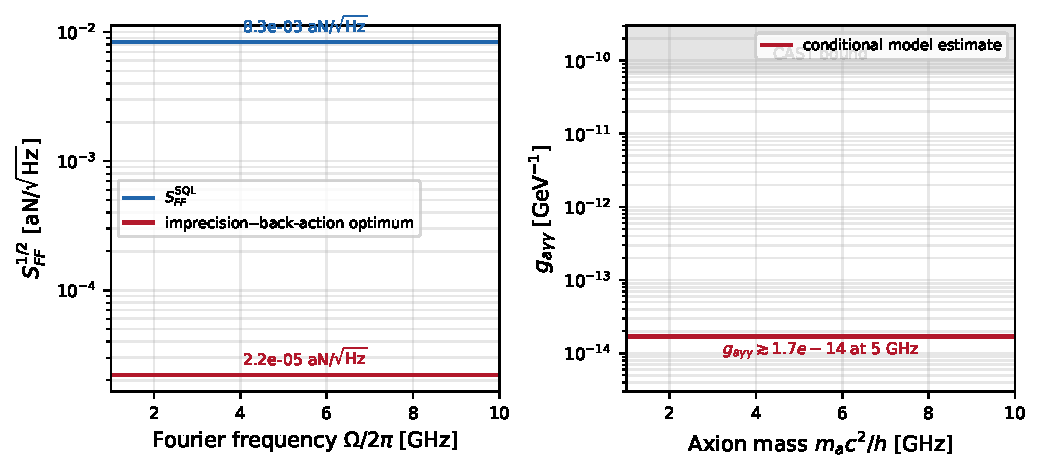
\includegraphics[width=0.8\columnwidth]{weak_force_limits.pdf}
\caption{Weak-force and axion projections at the deep-stability operating points (MacCabe platform parameters~\citep{MacCabe2020}). (a)~Force-noise scales referred to the mechanical port at $T_c=\qty{15}{\milli\kelvin}$: standard quantum limit $S_{FF}^{\rm SQL}=\sqrt{\hbar m_{\rm eff}\Omega_m\Gamma_m}=\qty{8.3e-3}{\atto\newton\per\sqrt{\hertz}}$ and imprecision--back-action optimum $S_{FF}^{\rm SQL}/\sqrt{\mathcal{C}/4}=\qty{2.2e-5}{\atto\newton\per\sqrt{\hertz}}$, both flat across the signal band for $\Omega\ll\Omega_m$. (b)~Conditional axion-photon coupling estimate for $B_0=\qty{10}{\tesla}$, $t_{\rm int}=\qty{1}{\hour}$, and $N=\num{12}$ under the bare model assumptions of the Supplemental Material, compared with the CAST solar-axion bound (shaded)~\citep{CAST2017}. No quantitative JPA-improved axion curve is claimed.}
\label{fig:weak_force_limits}
\end{figure}

\textit{Directional preamplification.} The marginal-stability class independently supplies net forward gain of $\qtyrange{13.5}{15.5}{\dB}$ with reverse isolation exceeding \qty{40}{\dB}, consistent with the Caves bound for a phase-preserving amplifier and comparable to gains reported for near-quantum-limited superconducting traveling-wave parametric amplifiers~\citep{Macklin2015}.

\textit{Instantaneous bandwidth.} Because the underlying dynamics are linear and the drift spectrum is sparse, the \qty{3}{\dB} detection bandwidth about the operating point is set by the smallest spectral gap to the imaginary axis, $\Delta\omega_{\rm 3dB}\approx|\max\Real\lambda|$ (heuristic estimate; values follow from the \cref{tab:nscaling} margins). Deep-stability solutions therefore support a bandwidth of order $\qty{0.7}{\kappa}$ ($\approx\qty{1.2}{\mega\hertz}$ on the MacCabe platform), while marginal-stability solutions are narrower ($\approx\qty{0.06}{\kappa}$). Both remain compatible with the \qtyrange{1}{10}{\giga\hertz} axion window once the mechanical resonance is tuned, the optical carrier providing the broadband conversion channel.

\section{Limitations}
\label{sec:limitations}

Eight boundaries delimit the present claims.
\begin{enumerate}
\item The optimized inter-chain couplings span the moderate range $\lint/J\in\numrange{0.07}{1.02}$; only the largest lattices operate in the perturbative weak-evanescent limit, and protection elsewhere is enforced empirically by the stability barrier ($\max\Real\lambda<\num{-0.05}$) rather than assumed perturbatively.
\item The Gaussian Lyapunov treatment assumes linear response, $\Delta\theta\ll\kappa$; larger signals would require nonlinear stochastic simulation.
\item The sub-attonewton force-sensing and axion projections presuppose dilution-refrigerator temperatures (so thermal occupation remains negligible) and, for the deep-stability class, a quantum-limited preamplifier; after inclusion of realistic added-noise numbers $n_{\rm add}\approx\num{0.5}$--$\num{1}$, the effective information remains $\Fnormeff\approx\num{0.3}$--$\num{0.5}$, still well above the single-port baseline.
\item The uncorrelated disorder study comprises 16 independent realizations at $\sigma_{\rm RMS}=\qty{5}{\percent}$; multi-restart DOC recovers $\ge\qty{80}{\percent}$ of nominal $\Fnorm$ in 14 of 16 cases (\qty{87.5}{\percent}). Larger ensembles would be required for tight confidence intervals.
\item Nine of the sixteen disorder realizations are retention-capped at \qty{200}{\percent}; the reported statistics therefore include this explicit capping and should be read as a conservative characterization.
\item The fast-scrambling diagnostics reported in the Supplemental Material are restricted to the early-time window $t\in\numrange{0.5}{1.5}\,\kappa^{-1}$ preceding boundary reflections and dissipative decay, set by the Duhamel error bound of \cref{SI-eq:si_duhamel}.
\item The effective non-reciprocal drift Hamiltonian requires high-frequency Floquet pump modulation ($\Omega_{\rm drive}\gg J,\kappa$); fast time-reversal switching (\cref{SI-fig:si_time_reversal}) demands flux-tunable couplers with sub-nanosecond switching times ($\tau_{\rm switch}\ll\kappa^{-1}$), stabilized in practice by the Kuramoto phase-locking mechanism of \cref{SI-eq:si_kuramoto}.
\item The projections onto force and axion sensitivity are illustrative of architectural reach under intermediate-coupling targets and are not claimed for present-day single-photon optomechanical couplings.
\end{enumerate}

\section{Conclusion}
\label{sec:conclusion}

A double-chain optomechanical ladder with opposing non-reciprocal hoppings yields a strictly positive resource-normalized Fisher information for every system size examined, once the total photon occupancy of both chains is taken into account as the metrological resource. The mechanism is spatial channel separation: the skin effect concentrates the signal at one boundary while the second chain drains quantum noise toward the opposite boundary. Differentiable optimal control reveals two complementary operating regimes that coexist as distinct basins of the non-convex landscape and sit at opposite ends of a continuous precision--gain frontier controlled by the spectral margin. One regime prioritizes per-photon precision at the cost of strongly attenuated forward transmission (and therefore requires a quantum-limited preamplifier, after which $\Fnormeff\approx\num{0.3}$--$\num{0.5}$ remains advantageous). The other supplies directional gain of order \qty{15}{\dB} at moderate normalized Fisher information. Every optimized solution remains Hurwitz-stable under moderate fabrication disorder, and multi-restart re-optimization restores at least \qty{80}{\percent} of nominal precision in a majority of disordered realizations. Within the stated linear-response, two-chain Gaussian model and full photon accounting, the architecture supplies a concrete multi-port route past the single-port Petermann bound, while making the associated precision--gain trade-off quantitative and experimentally addressable. The claim is falsifiable by a single test: two-chain photon-counted homodyne $\Fnorm$ versus single-chain at matched total occupancy, with the readout added-noise number stated.

\section*{Supplemental Material}

See Supplemental Material at [URL will be inserted by publisher] for the theoretical framework, the single-chain benchmark, the double-chain ladder parameters and solution classes, the disorder-resilience study, the initialization-resampling characterization, the OTOC and cutoff-convergence diagnostics, the weak-force and axion projections, and the scope boundaries.

\section*{Data availability}

The data that support the findings of this study are available within the article and its Supplemental Material. Manuscript sources, deterministic analysis scripts, and the environment specification are publicly archived at \url{https://github.com/NanaEngo/floquet-nhse-synthetic-flux}.

\section*{Acknowledgments}

We thank the Stellenbosch Institute for Advanced Study for hospitality. Computational resources were provided by the penavoraserver cluster (ThinkStation P720, 128 GB RAM, 48 cores) through Penabei Samafou; supporting data are provided with the manuscript. This work received no external funding.

\section*{Author contributions}

JD and PD performed the numerical simulations and analyzed the data. AHAA, AE, NM contributed to the theoretical framework and provided critical feedback on the results. SGNE conceived and supervised the project, directed the research. PD and SGNE wrote the final version of the manuscript. All authors reviewed and approved the final manuscript.

\section*{Competing interests}

The authors declare no competing interests.

\section*{Use of AI}

AI-based language models were used to support literature searches, to refine and debug analysis scripts, and to check DOIs and bibliographic information. All AI-generated content was verified and edited by the authors, who remain fully responsible for the manuscript. All authors remain responsible for the accuracy, originality, interpretation, and final wording of this manuscript.

\bibliographystyle{apsrev4-2}
\bibliography{references}

\end{document}
